%%%%%%%%%%%%%%%%%%%%%%%%%%%%%%%%%%%%%%%%%

%%%%%%%%%%%%%%%%%%%%%%%%%%%%%%%%%%%%%%%%%

%----------------------------------------------------------------------------------------
%	PACKAGES AND DOCUMENT CONFIGURATIONS
%----------------------------------------------------------------------------------------

\documentclass[https://www.overleaf.com/project/63761df255a8a9f4a15c3579
	letterpaper, % Paper size, specify a4paper (A4) or letterpaper (US letter)
	10pt, % Default font size, specify 10pt, 11pt or 12pt
]{CSUniSchoolLabReport}


\usepackage{hyperref}
\usepackage[normalem]{ulem}
\usepackage{listings}
\usepackage{xcolor}
\definecolor{codegreen}{rgb}{0,0.6,0}
\definecolor{codegray}{rgb}{0.5,0.5,0.5}
\definecolor{codepurple}{rgb}{0.58,0,0.82}
\definecolor{backcolour}{rgb}{1,1,1}
\lstdefinestyle{mystyle}{
    backgroundcolor=\color{backcolour},   
    commentstyle=\color{codegreen},
    keywordstyle=\color{magenta},
    numberstyle=\tiny\color{codegray},
    stringstyle=\color{codepurple},
    basicstyle=\ttfamily\footnotesize,
    breakatwhitespace=false,         
    breaklines=true,                 
    captionpos=b,                    
    keepspaces=true,                 
    numbers=left,                    
    numbersep=5pt,                  
    showspaces=false,                
    showstringspaces=false,
    showtabs=false,                  
    tabsize=2
}

\lstset{style=mystyle}
\renewcommand\ULthickness{1.0pt}   %%---> For changing thickness of underline
\setlength\ULdepth{1.3ex}%\maxdimen ---> For changing depth of underline

%----------------------------------------------------------------------------------------
%	REPORT INFORMATION
%----------------------------------------------------------------------------------------


\begin{document}

\begin{figure}[H] % [H] forces the figure to be placed exactly where it appears in the text
	\centering % Horizontally center the figure
	
\includegraphics[width=0.4\textwidth]{Figures/logo.png} % Include the figure
\end{figure}

\begin{center}
	\begin{tabular} {c}
        \Huge Universidad La Salle \\\\\\\\
		\huge Fundamentos de Lenguajes de Programación \\\\\\\\
		\LARGE Informe \\\\\\\\
        \huge Una Comparación entre C++, Go y Python \\\\\\\\
        \LARGE Karlo Emigdio Pacha Curimayhua \\\\\\\\
        \LARGE Quinto Semestre - Ingeniería de Software \\\\\\\\
		\LARGE 2022
	\end{tabular}
\end{center}

\begin{center}
	\begin{tabular}{l r}
	\end{tabular}
\end{center}



% If you need to include an abstract, uncomment the lines below
%\begin{abstract}
%	Abstract text
%\end{abstract}

%----------------------------------------------------------------------------------------
%	Introducción
%----------------------------------------------------------------------------------------

\section{Introducción}

Go es un lenguaje de programación compilado basado en C (en el aspecto sintáctico) y parecido a Python al momento del dinamismo que posee. El objetivo de este trabajo es poner a prueba los 3 lenguajes mencionados con los algoritmos de ordenamiento: Cocktail Sort y Counting Sort.
 
%----------------------------------------------------------------------------------------
%	Algoritmos
%----------------------------------------------------------------------------------------

\section{Algoritmos}

\subsection{Cocktail Sort}

Es un algoritmo de ordenamiento con complejidad cuadrática \(O(n^2)\) como se puede apreciar en la Tabla 1; este es una variación del Bubble Sort que recorre la lista de datos en ambas direcciones de forma alternativa (al contrario que el Bubble Sort que sólo lo hace en una dirección). \\
Los pasos son:\\

\begin{center}
    \begin{tabular}{| c | c |}
        \hline
            Caso & Complejidad \\ 
        \hline
            Mejor caso & \(O(n)\) \\
            Caso promedio & \(O(n^2)\) \\
            Peor caso & \(O(n^2)\) \\ 
        \hline
    \end{tabular}
\end{center}

 \begin{center}
    Tabla 1 : Complejidad Temporal
 \end{center}

\begin{tabular}{lr}
    I. El primer paso es recorrer la lista de datos de izquierda a derecha, se comparan \\
    los valores adyacentes, y si el valor de la izquierda es mayor, se intercambian los \\
    valores. El objetivo es poner el valor máximo al final.\\\\

    II. El segundo paso es recorrer la lista de datos de derecha a izquierda, se \\
    comparan los valores adyacentes, y si el valor de la derecha es menor, se intercambi-\\
    an los valores. El objetivo es poner el valor mínimo al inicio.\\\\
\end{tabular}

Este proceso continúa hasta que los elementos de la matriz no se ordenan.\\


\subsection{Counting Sort}

Es un algoritmo de ordenamiento con complejidad  \(O(n + k)\), esta aplica para todos los casos como se puede apreciar en la Tabla 2; este algoritmo basa su funcionamiento en los índices, no en comparaciones como los demás. Este algoritmo depende mucho del elemento con el valor máximo. \\


\begin{center}
    \begin{tabular}{| c | c |}
        \hline
            Caso & Complejidad \\ 
        \hline
            Mejor caso & \(O(n + k)\) \\
            Caso promedio & \(O(n + k)\) \\
            Peor caso & \(O(n + k)\) \\ 
        \hline
    \end{tabular}
\end{center}

 \begin{center}
    Tabla 2 : Complejidad Temporal
 \end{center}

Los pasos son:\\

\begin{tabular}{lr}
    I. Busca el elemento máximo (max) y el mínimo (min).\\\\
    II. Crea una lista auxiliar de tamaño max + 1.\\\\
    III. Se subdivide en los siguientes pasos:\\\\
    \begin{tabular}{lr}
        - Se almacena el recuento de cada elemento de la lista en su índice correspon-\\
        diente en la lista auxiliar.\\\\
        - Se suman los recuentos (a[i] + a[i-1]]), esto para colocar los elementos en \\
        el índice correcto de la lista ordenada.\\\\
    \end{tabular}
    \\IV. Posiciona los elementos en la lista original o una de salida, para esto se utilizan los índices.\\\\
\end{tabular}

El punto débil de este algoritmo es la complejidad espacial O(max), si el elemnto de mayor valor tiene un número de dígidos superior al tamaño de la lista de datos, el costo es casi cuadrático.\\


%----------------------------------------------------------------------------------------
%	Implementación
%----------------------------------------------------------------------------------------

\section{Implementación}

Para poner a prueba los algoritmos de Cocktail y Counting Sort, se necesitan varios archivos CSV que contengan entre: 100, 1000, 2000, 3000, 4000, 5000, 6000, 7000, 8000, 9000, 10000, 20000, 30000, 40000 y 50000 datos. \\\\
Una vez se implementen los algoritmos en los 3 lenguajes, se ejecutarán con cada lista de datos generada, por cada tamaño se ejecutará y medirá el tiempo de ejecició (en segundos) 5 veces y luego se obtendrá un promedio. \\\\
Finalmente, los datos obtenidos se exportarán en un CVS.

\subsection{Generador C++}
\lstinputlisting[language=Octave]{codes/generator.cpp}

\subsection{Cocktail Sort C++}
\lstinputlisting[language=Octave]{codes/CocktailSort.cpp}

\subsection{Cocktail Sort Go}
\lstinputlisting[language=Octave]{codes/CocktailSort.go}

\subsection{Cocktail Sort Python}
\lstinputlisting[language=Octave]{codes/CocktailSort.py}

\subsection{Counting Sort C++}
\lstinputlisting[language=Octave]{codes/CountingSort.cpp}

\subsection{Counting Sort Go}
\lstinputlisting[language=Octave]{codes/CountingSort.go}

\subsection{Counting Sort Python}
\lstinputlisting[language=Octave]{codes/CountingSort.py}

\subsection{Graficador Python}
\lstinputlisting[language=Octave]{codes/grapher.py}

%----------------------------------------------------------------------------------------
%	Resultados
%----------------------------------------------------------------------------------------

\section{Resultados}
%----------------------------------------------------------------------------------------
\subsection{Tabla Comparativa: Cocktail Sort}

\begin{figure}[H] 
	\centering 
	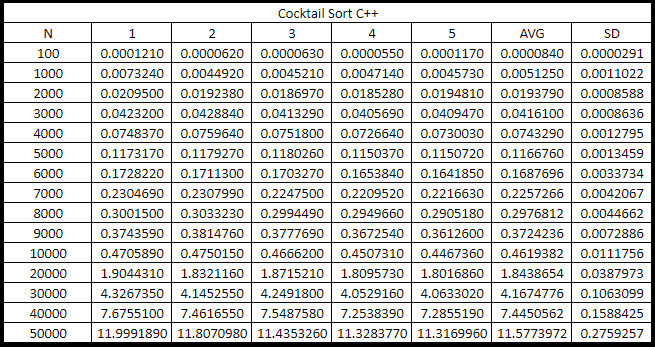
\includegraphics[width=1\textwidth]{Figures/1.png} % Include the figure
\end{figure}
\begin{center}
    Tabla 3 : Tiempos de ejecución, promedio y desviación estándar
\end{center}
 
\begin{figure}[H] 
	\centering 
	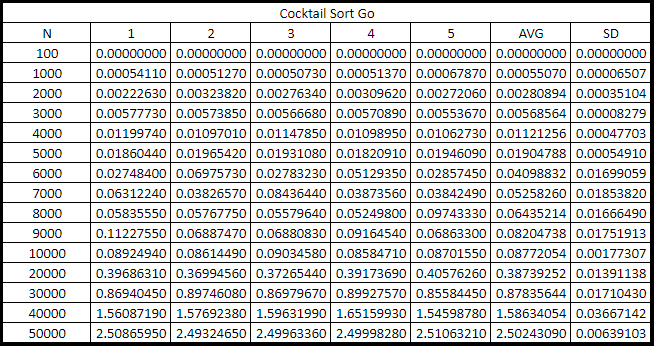
\includegraphics[width=1\textwidth]{Figures/2.png} % Include the figure
\end{figure}
\begin{center}
    Tabla 4 : Tiempos de ejecución, promedio y desviación estándar
\end{center}

\begin{figure}[H] 
	\centering 
	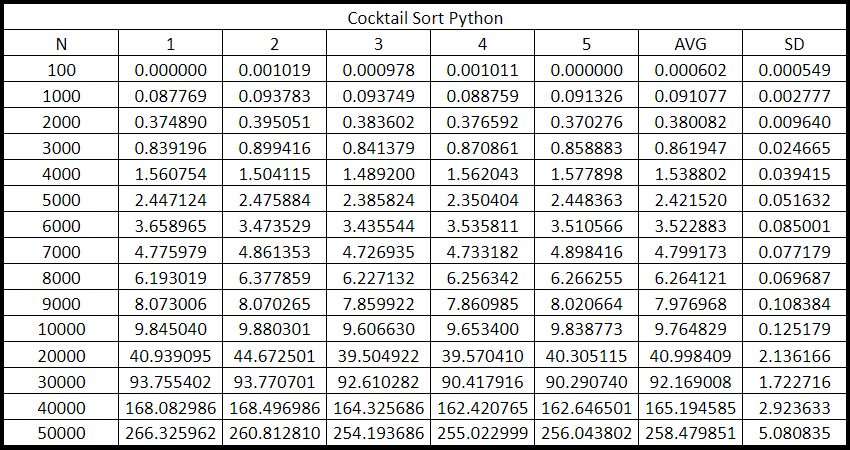
\includegraphics[width=1\textwidth]{Figures/3.png} % Include the figure
\end{figure}
\begin{center}
    Tabla 5 : Tiempos de ejecución, promedio y desviación estándar
\end{center}

%----------------------------------------------------------------------------------------
\subsection{Tabla Comparativa: Counting Sort}

\begin{figure}[H] 
	\centering 
	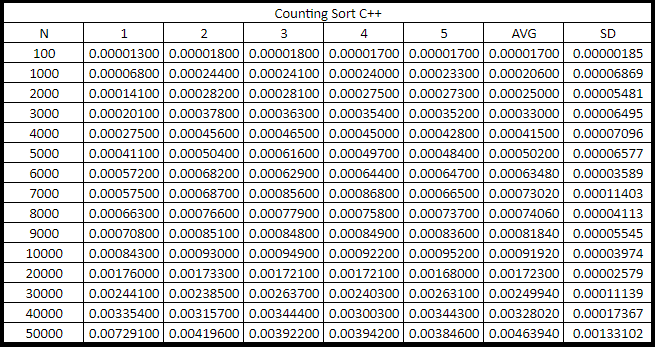
\includegraphics[width=1\textwidth]{Figures/4.png} % Include the figure
\end{figure}
\begin{center}
    Tabla 4 : Tiempos de ejecución, promedio y desviación estándar
\end{center}

\begin{figure}[H] 
	\centering 
	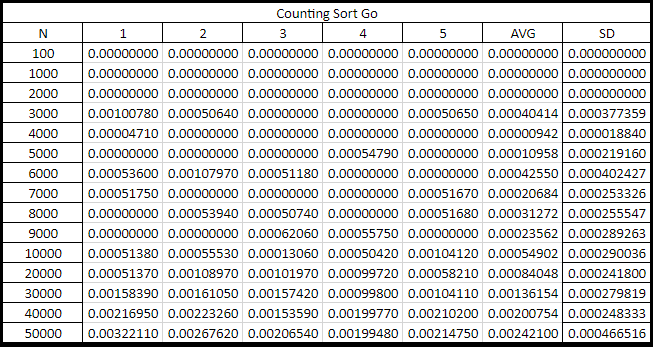
\includegraphics[width=1\textwidth]{Figures/5.png} % Include the figure
\end{figure}
\begin{center}
    Tabla 5 : Tiempos de ejecución, promedio y desviación estándar
\end{center}

\begin{figure}[H] 
	\centering 
	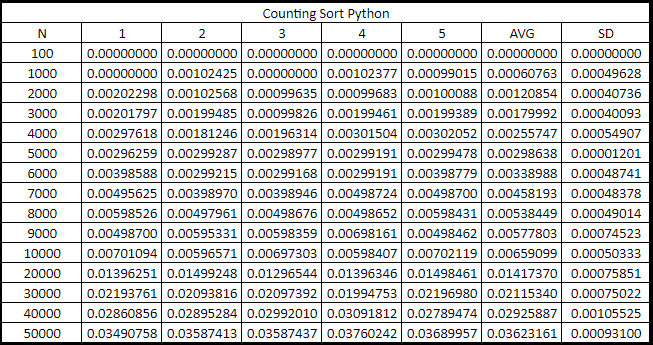
\includegraphics[width=1\textwidth]{Figures/6.png} % Include the figure
\end{figure}
\begin{center}
    Tabla 6 : Tiempos de ejecución, promedio y desviación estándar
\end{center}

%----------------------------------------------------------------------------------------
\subsection{Gráfico Comparativo: Cocktail Sort}

\begin{figure}[H] 
	\centering 
	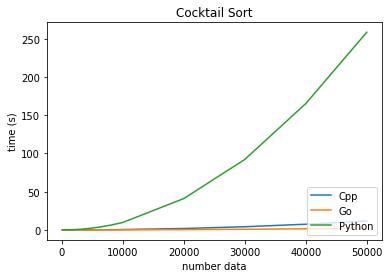
\includegraphics[width=0.9\textwidth]{Figures/cocktailSort.png} % Include the figure
	\caption{Cocktail Sort en C++, Go y Python}
\end{figure}

\begin{figure}[H] 
	\centering 
	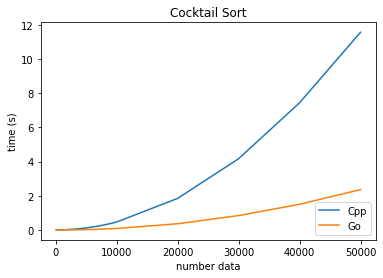
\includegraphics[width=0.8\textwidth]{Figures/cocktailSort2.png} % Include the figure
	\caption{Cocktail Sort en C++ y Go}
\end{figure}

Como se ve en la  Figura 1, Python es uno de los peores lenguajes en lo que rendimiento respecta (esto debido a su naturaleza [interpretado]). A pesar de que C++ suele ser el mejor en tiempo de ejecución, esta vez Go es superior. \\\\
Si sólo se examina la Figura 1, parece que la diferencia no es tan amplia, pero en la Figura 2, se ve que Go tuvo un tiempo de ejecución notablemente mejor, se toma casi la mitad del tiempo que se toma C++.

%----------------------------------------------------------------------------------------
\subsection{ Gráfico Comparativo: Counting Sort}

\begin{figure}[H] 
	\centering 
	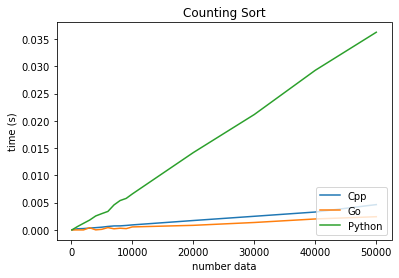
\includegraphics[width=0.8\textwidth]{Figures/countingSort.png} % Include the figure
	\caption{Counting Sort en C++, Go y Python}
\end{figure}

\begin{figure}[H] 
	\centering 
	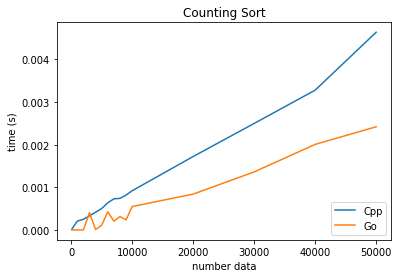
\includegraphics[width=0.9\textwidth]{Figures/countingSort2.png} % Include the figure
	\caption{Counting Sort en C++ y Go}
\end{figure}

Si se examina la Figura 3, Python sigue mostrando un mal rendimiento, sigue teniendo una grna diferencia con Go y C++. Nuevamente Go se moetró superior a C++. \\\\
Al examinar la Figura 4, se puede notar que Go ya no fue tan superior a C++, incluso en un punto fue mejor. Esta vez la diferencia sería de un t - C, donde C es casi igual a 0.0005 segundos, aunque este se va incrementando.

%----------------------------------------------------------------------------------------
%	Conclusiones
%----------------------------------------------------------------------------------------

\section{Conclusiones}

Realmente no se podría concluir algo claro con los resultados del experimento, a pesar de que parece que Go es mejor que C++, esto debido a las tablas de los tiempos obtenidos, se puede apreciar que Go y Python en los primeros casos dan como resultado 0, lo cual no puede ser posible incluso en el Counting Sort, C++ no retorna 0 en tiempos de ejecución. 
Una vez expuesto esto, se podría decir que Go y Python no capturaron el tiempo de ejecución de la mejor forma, podría ser esa la razón por la que C++ se mostró inferior a Go. \\\\
Una vez aclarado la "victoria" de Go sobre C++, se puede decir que los lenguajes de programación compilados son claramente superiores a los interpretados, o incluso a los que están en un punto intermedio como es el caso de Java. Esta es la principal razón por la que estos se usan para la base de sistemas grandes y con una gran cantidad de opraciones, es la razón de la existencia de TypeScript y Numba que tiene como objetivo mejorar JavaScript y Python respectivamente. Pero esto no quiere decir que los lenguajes interpretados no tengan uso (de hecho son los más utilizados), pero si se ven limitados para casos de exigencia máxima  \\\\\\


%----------------------------------------------------------------------------------------

\href{https://github.com/KEPCU/FundamentalsOfProgrammingLanguages/tree/master/go/practice16}{GitHub} : \url{https://github.com/KEPCU/FundamentalsOfProgrammingLanguages/tree/master/go/practice16}

%----------------------------------------------------------------------------------------

\end{document}